
%
\documentclass[journal]{IEEEtran}
\usepackage{blindtext}
\usepackage{graphicx}
\usepackage{booktabs}
\usepackage[cmex10]{amsmath}

% *** GRAPHICS RELATED PACKAGES ***
%
\ifCLASSINFOpdf
 
\else
 
\fi

\hyphenation{op-tical net-works semi-conduc-tor}


\begin{document}

\title{Exchange Rate Forecasting using Ensemble Artificial Neural Network Model }

\author{Wut Hmone Hnin Hlaing, whlaing10@gmail.com, Faculty of Computing \& Informatics, Multimedia University, Cyberjaya}
	%
% make the title area
\maketitle

\begin{abstract}
Artificial Neuron Network (ANN) is one of the methods which has been widely used in forecasting the financial market.  In this project, an ensemble ANN model is used to forecast the currency exchange rate between Malaysian Ringgit and other currencies. The ensemble ANN models are constructed with homogeneous neural networks such as Multi-layer Perceptrons (MLPs) using different algorithms and also with heterogeneous neural networks such as MLPs, Recurrent Neural Network (RNN), and Radial Basis  Function network (RBF). The models are trained three different training ratio, such as 80\%,70\%, and 60\% for six different currencies such as USD, EUR, GBP, AUD, SGD and CHF. The performance of the models are compared against each other. The project concludes that the homogeneous ensemble which trained with 60\% training inputs data yield the best accuracy performance for all the currencies.
\end{abstract}

\begin{IEEEkeywords}
 ANN, ensemble method, forecasting, Malaysian Ringgint, MLP, RNN, RBF 
\end{IEEEkeywords}


\IEEEpeerreviewmaketitle

\section{Introduction}
Exchange rates can be defined as the values which are used for  converting one currency to another currency. Exchange rates are influenced by many factors such as economic situations and political changes, and also the psychological states of individual  who involved in trading and investing in the financial markets.Forecasting the exchange rates is not a simple task due to its complex correlations with the factors that influenced by. Their interactions are complex, dynamic and  unstable  manners.There are many approaches exist for forecasting exchange rates.  This project mainly focuses on technical  analysis approach. Technical analysis approach performs the prediction by analyzing the past behaviors of the data and, identifying the patterns within it, and makes the predictions on the  behaviors  in the future.
\section{Artificial Neural Network}

A biological neuron consists of an axon, synapse, and dendrite. The inputs in biological  neuron come along by dendrite to the synapses,and when it reaches  the certain value or threshold, in other words, it fires,  and the outputs are transmitted  to another neuron. Each neuron in the brain receives several inputs and produce  an output. The inputs  are summed up to give the total input to the unit. Based on the biological neuron, the functions of a single neuron can be summarized by Beale and Jackson[1] as:
\begin{itemize}
	\item The output from a neuron is either on or off.
	\item The output depends only on the inputs, and it  needs to reach a certain number in order to make the neuron fire.
\end{itemize}

An artificial neuron constructs based on the basic functions of  a biological brain. In order to reach the limit or threshold,  the weights are added in construction the artificial neurons. After summation of inputs and weights, the results  to the  transfer functions . This artificial neuron model was proposed by McColloch and Pitts. In their model, threshold activation function was applied.


\subsection{Time Series Forecasting with ANNs}

Time series forecasting involves using the available data and using it to predict the future values of this series. Forecasting exchange rates can be considered as time series forecasting. In the project,  the forecasting  is made by using ensemble ANNs model or network.

In time series forecasting, there are two types of forecasting methods which can apply. They are the single-step prediction and iterated single-step prediction or  multi-step prediction. For single-step prediction, the network is trained with several hundred of data vectors each consisting of such four days data, along with a fifth one which is the target. When the network is trained, a vector for observations of four days are supplied, and the network produces an output for the fifth day. 

Multi-step prediction is used when a long-term prediction is required. In multi-step prediction, the predicted output is fed back as input for the next forecasting and all other input units are shifted back one unit. Hence, the inputs consist of predicted values as well the original  time series data.

\subsection{Learning Paradigms}

The two learning paradigms for the neural network  are supervised and unsupervised learning.

In the supervised learning paradigm, the correct or right answers are given to the network. This type of approach  has the  knowledge of targeted outputs or desired results. It is given by many examples of the problem to train. The neural network tires and generalizes the underlying rules of the problem  during the training process. In this approach, the neural network is given a problem, to make a forecasting. This forecasting is then compared to the desired output or correct outputs which are given to the network during the training process. The learning algorithm utilizes the error information to correct the weights of  the neural network so that the next time the forecasting will be closer to the correct answer. Since the neural network learns by looking at examples, the number of examples provided has to be large enough for effective training. 

In the unsupervised learning paradigm, the neural network is asked to figure things out for itself. Unlike the supervised learning, it is not given the correct answers. The network only given the inputs data.  The task of the neural network is to look at the patterns of data and to cluster them so that similar patterns get put in the same cluster. Self-organizing networks are one of the categories of unsupervised learning because they don't have the knowledge about the desired or correct output should be. 

This project  is based on supervised learning paradigm. The neural network is supplied historical exchange rates and learns to recognize patterns from these inputs. Since the neural network knows the output of the data set, the training continues until the network is able to match the data with sufficient accuracy.

\section{Literature Review}

During recent decades, many kinds of literature have been developed in the area of neural networks methods. Many applications apply ANNs methods  to forecast in different fields such as medical diagnostics, general business, financial markets and so on. ANNs methods  are popular because of the ability to generalize and learn from training process or experiences. Forecasting is one of the first successful areas which applied ANNs techniques which is also known as nonlinear techniques. 

It the paper, Hansen(1992) showed that simple ensembles can perform better generalizations than a single ANN and that a subset of all possible ANNs can achieve better results than a single ANN. Moreover, Hiacomel(2015) constructed the ensemble ANNs network by using two ANNs  architectures  with a different number of nodes, input layers, hidden layers, and outputs layers to predict financial time series market. The research shows that the ensemble ANNs  network outperformed the single ANN network model. Their ensemble has shown itself not as a tool that always gets the best profits, but instead gives good and consistent results.


In the paper of Ppacelli(2011), they made two hypotheses to valid using ANNs networks. They tried to validate that : the financial markets pricing process  is not random, and the degree of information efficiency of the financial markets is not strong or semi-strong. Their ANNs was built by using MLPs methods. Their research found that the dependence of prices in financial markets is not completely random, and therefore, it can be predictable.

In their paper Hua(2010), to predict the exchange rate, they used ANNs methods, and Kernel Regression methods, to smooth the noise. The research tried to predict for the three different exchange rates, one, three, and twelve months ahead by using training data sets of US to British Pound exchange rates, Indian Rupees, and Japanese Yen. They compared their methods to traditional statistical forecasting methods and found that their ANNs with Kernel Regression methods outperformed the traditional

Besides, Adhikari(2013) showed in their paper that accuracies of the ANN forecasting are significantly better and improved  through ensemble method. It is  showed that this combined training algorithm performs much better than each of the individual ones. However, methodologies based on single ANN method have been largely used for financial time series prediction while ANNs ensembles are still little used in this area. Hence, this project plans to apply ensembles ANNs methods to forecast the exchange rates.
Radial basis function neural networks (RBF)are also applied in different fields. Sermpinis(2013) has done a study which forecasted the exchange rates by using RBF neural network functions. It is shown that the neural networks methods produced better results compared to statistical linear models.

All the above paper  constructed by using single ANN methods or technique. It has been shown the accuracy of the results is much better with  ensemble ANNs methods. Ensemble ANNs networks are constructed by combining two or more ANNs methods, or by applying different kinds of learning algorithms to train the dataset, or using the two or more same  ANNs network as a combination network.

It the paper, Hhansen(1992)  showed that simple ensembles can perform better generalizations than a single ANN and that a subset of all possible ANNs can achieve better results than a single ANN. Moreover, Giacomel(2015) constructed the ensemble ANNs network by using two ANNs  architectures  with a different number of nodes, input layers, hidden layers, and outputs layers to predict financial time series market. The research shows that the ensemble ANNs  network outperformed the single ANN network model. Their ensemble has shown itself not as a tool that always gets the best profits, but instead gives good and consistent results.

Ensemble ANNs methods produce  better performance not only in forecasting the exchange rates but also in the different research fields. Shao(2014) built an ensemble ANNs network for fault diagnosis of proton exchange membrane fuel cell system. It showed that this method can improve the accuracy to 93.24\%, and greatly reduce failure  to report in fault diagnosis, while the accuracies of single  ANN network applied to  have  only the interval from 75.24\% to 85.62\%.

As for the Malaysian Ringgits and USD currency exchange rates, Chan(2010) conducted a reasearch on whether using ANNs model will give the desirable accuracy outputs. In their paper, the results mentioned that ANNs models outperformed the random walks model and, produced the desirable accuracy for the prediction with is 0.02065 RMSE error rate.

\section{Ensemble ANNs Model Design}

Two type of ensemble networks is constructed using this model which are homogeneous ensemble model, and  heterogeneous ensemble model. As for the homogeneous ensemble model, the NN1, NN2, and NN3 is implemented using the same network, MLPs by using different activation functions and learning functions. As for heterogeneous ensemble model, the NN1, NN2, and NN3 is implemented using different ANNs methods such as MLPs, RNN, and RBF neural network. Different type of fusion functions is applied to both model such as average function, minimum function, and maximum function.

The number of inputs is planned to start with prediction order three and increased to ten. The number of hidden layers and hidden nodes is carefully selected  after an extensive review of the previous literature. These network topology is applied to forecast  USD, EUR, GBP, SGD, AUD, CHF to Malaysian Ringgint (RM). The outputs from NN1, NN2, and NN3 is used to finalize by using an average function. Fig 1. explains the model in graphical manner.

\begin{figure}[hbt!]\centering
	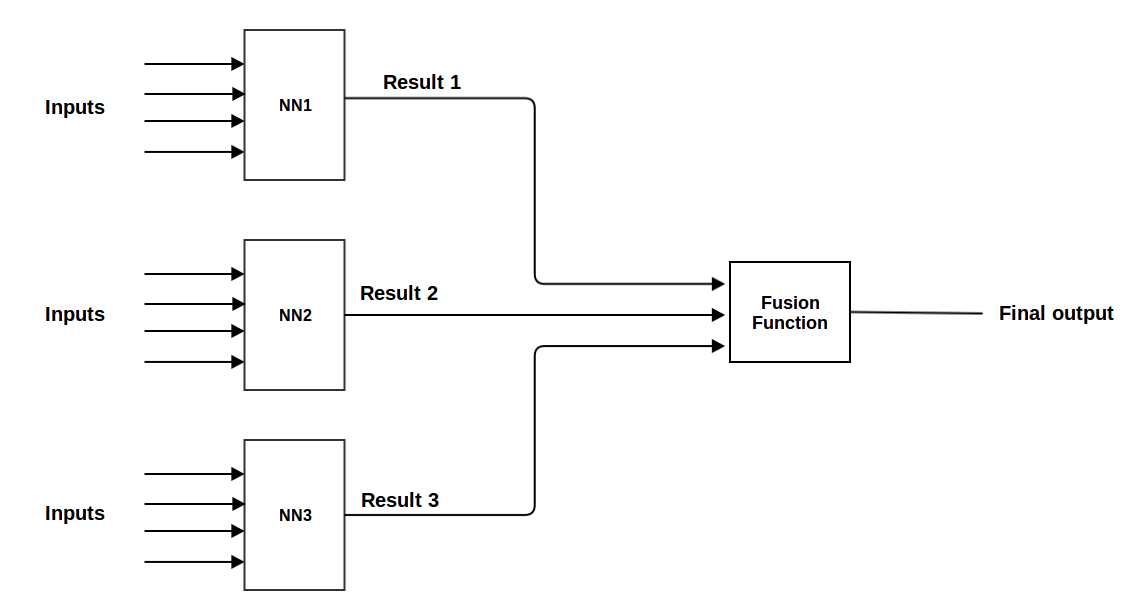
\includegraphics[width=0.5\textwidth]{ensemblemodel}
	\caption{The proposed ensemble ANNs model}
\end{figure}


\subsection{Performance Measurements}

There are many methods which measure the accuracy of the neural network by calculating the errors between actual outputs and forecasted outputs by the neural networks. There are many methods to calculate the errors. The most widely used methods are mentioned with their mathematical equation.
\\
\\
\textbf{Root Mean Squared Error (RMSE)}\\
\begin{equation*}
	RMSE= \sqrt{\frac {1}{n}\sum_{i=0}^n(forecasted -  actual )^2} 
\end{equation*}

\textbf{Mean Absolute Error(MAE)}\\
\begin{equation*}
	MAE= \frac {1}{n} \sum_{i=0}^n (forecasted - actual)
\end{equation*}

\section{Research Findings}	


The optimal two ensemble models for the USD, EUR, GBP, SGD, AUD, and CHF to RM exchange rate are shown together with the training ratio that yield the optimal models and their predictor order, RMSE, MAE, activation function, learning rate, and fusion function applied.

\begin{table}[ht]
	\centering
	\begin{tabular}{@{}rrrrrrrrrr@{}}
		\toprule
		\textbf{Model} &\textbf{PO}&\textbf{Neurons}& \textbf{RMSE} & \textbf{MAE} & \textbf{Act\_F} & \textbf{LR} \\
		\midrule
		
		HOMO	& 9 & 9 & 0.012598 & 0.009269 & tanh & 0.1 \\ 	
		HETERO	& 3 & 17 & 0.012704 & 0.009321 & tanh & 0.1  \\
		MLP	&  9 & 9 & 0.012717 &  0.009399 & tanh & 0.1 \\	
		RNN	&  9 & 9 & 0.034810 &  0.026693 & tanh & 0.1 \\
		RBF	&  9 & 9 & 0.050619 & 0.045792 & tanh & 0.1  \\
		\hline
	\end{tabular}
	\hspace*{3cm}
	\caption{The model performance for USD to RM }
\end{table}

\begin{table}[ht]
	\centering
	\begin{tabular}{@{}rrrrrrrrrr@{}}
		\toprule
		\textbf{Model} &\textbf{PO}&\textbf{Neurons}& \textbf{RMSE} & \textbf{MAE} & \textbf{Act\_F} & \textbf{LR} \\
		\midrule
		
			HOMO	& 3 & 8 & 0.019116 & 0.014616 & tanh & 0.1  \\ 	
			HETERO	&3 & 3 & 0.019668 & 0.015139 & tanh & 0.1  \\
			MLP	& 3 & 8 & 0.019824 &  0.015608 & tanh & 0.1 \\	
			RNN	&  3 & 8 & 0.041590 & 0.035251 & tanh & 0.1 \\
			RBF	& 3 & 8 & 0.030003 & 0.0238661 & tanh & 0.1  \\
		\hline
	\end{tabular}
	\hspace*{3cm}
	\caption{The model performance for EUR to RM }
\end{table}

\begin{table}[ht]
	\centering
	\begin{tabular}{@{}rrrrrrrrrr@{}}
		\toprule
		\textbf{Model} &\textbf{PO}&\textbf{Neurons}& \textbf{RMSE} & \textbf{MAE} & \textbf{Act\_F} & \textbf{LR} \\
		\midrule
		
		HOMO	& 3 & 6 & 0.022409 & 0.016851 & tanh & 0.1 \\
		HETERO	&4 & 6 & 0.022505 & 0.016948 & tanh & 0.1  \\ 
		MLP	&  3 & 6 & 0.022430 &  0.016852 & tanh & 0.1 \\	
		RNN	& 3 & 6 & 0.056163 & 0.049153 & tanh & 0.1 \\
		RBF	& 3 & 6 & 0.040494 & 0.030088 & tanh & 0.1  \\
		\hline
	\end{tabular}
	\hspace*{3cm}
	\caption{The model performance for GBP to RM }
\end{table}


\begin{table}[ht]
	\centering
	\begin{tabular}{@{}rrrrrrrrrr@{}}
		\toprule
		\textbf{Model} &\textbf{PO}&\textbf{Neurons}& \textbf{RMSE} & \textbf{MAE} & \textbf{Act\_F} & \textbf{LR} \\
		\midrule
		
		HOMO	&  3 & 5 & 0.006562 & 0.004605 & tanh & 0.1 \\
		HETERO	& 3 & 5 & 0.006692 & 0.004687 & tanh & 0.1  \\  
		MLP	&  3 & 5 & 0.006596 & 0.004628 & tanh & 0.1 \\	
		RNN	& 3 & 5 & 0.034397 & 0.028842 & tanh & 0.1 \\
		RBF	& 3 & 5 & 0.043879 & 0.040975 & tanh & 0.1  \\
		\hline
	\end{tabular}
	\hspace*{3cm}
	\caption{The model performance for SGD to RM }
\end{table}


\begin{table}[ht]
	\centering
	\begin{tabular}{@{}rrrrrrrrrr@{}}
		\toprule
		\textbf{Model} &\textbf{PO}&\textbf{Neurons}& \textbf{RMSE} & \textbf{MAE} & \textbf{Act\_F} & \textbf{LR} \\
		\midrule
		
			HOMO	& 9 & 5 & 0.015048 & 0.011326 & tanh & 0.1  \\ 
			HETERO	& 3 & 17 & 0.015111 & 0.011378 & tanh & 0.1  \\  
		MLP	&  3 & 5 & 0.015056 & 0.011391 & tanh & 0.1 \\	
		RNN	&  3 & 5 & 0.048412 & 0.036032 & tanh & 0.1 \\
		RBF	&  3 & 5 & 0.038108 & 0.032192 & tanh & 0.1  \\
		\hline
	\end{tabular}
	\hspace*{3cm}
	\caption{The model performance for AUD to RM }
\end{table}

	
\begin{table}[ht]
	\centering
	\begin{tabular}{@{}rrrrrrrrrr@{}}
		\toprule
		\textbf{Model} &\textbf{PO}&\textbf{Neurons}& \textbf{RMSE} & \textbf{MAE} & \textbf{Act\_F} & \textbf{LR} \\
		\midrule
		
		HOMO	& 9 & 6 & 0.017436 & 0.012879 & logistic & 0.1  \\
		HETERO	&  8 & 18 & 0.017514 & 0.012996 & tanh & 0.1 \\  
		MLP	& 9 & 6 & 0.017722 & 0.013076 & tanh & 0.1 \\	
		RNN	&  9 & 6 & 0.031643 & 0.024210 & tanh & 0.1 \\
		RBF	& 9 & 6 & 0.039575 & 0.0317153 & tanh & 0.1  \\
		\hline
	\end{tabular}
	\hspace*{3cm}
	\caption{The model performance for CHF to RM }
\end{table}

For all the currencies, the models with trained with 60\% training inputs yield the best accuracy performance for both homogeneous and heterogeneous ensemble model.


The performance comparison for both ensemble model based on the RMSE performance demonstrated in the Fig 2.  
\begin{figure}[hbt!]\centering
	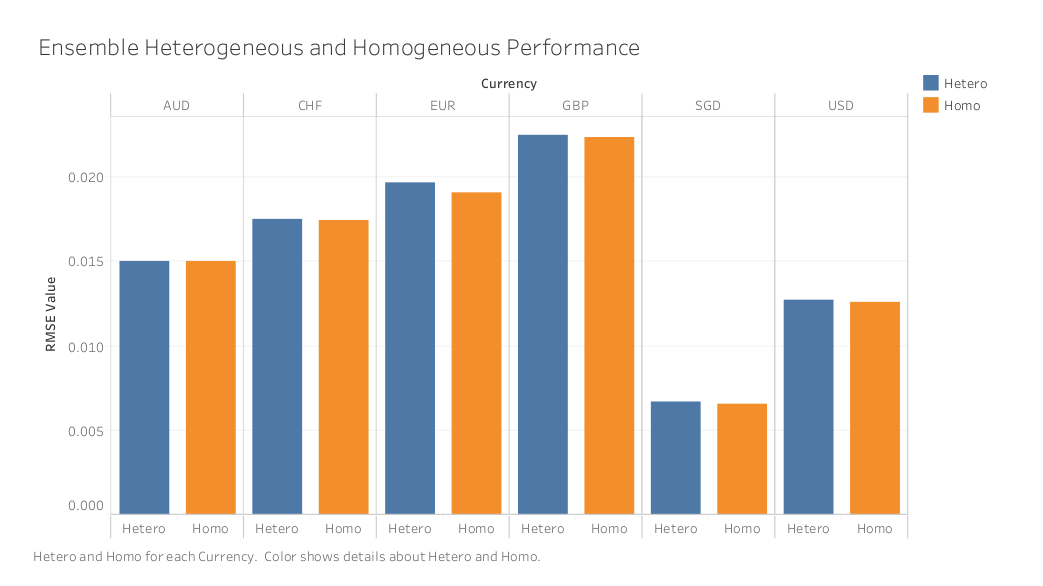
\includegraphics[width=0.5\textwidth]{compare_homo_hetero}
	\caption{Comparison between optimal Ensemble Heterogeneous and Homogeneous Model}
\end{figure}

It can be said that both models yield the similar performance, but homogeneous ensemble model outperformed the heterogeneous model.

These two ensemble model are compared with the single models performance as well. It is found that the ensemble models outperformed the single models, and the MLP single model yield the best performance for the single models for every currency. The Fig. 3 explained their performance comparison.


\begin{figure}[hbt!]\centering
	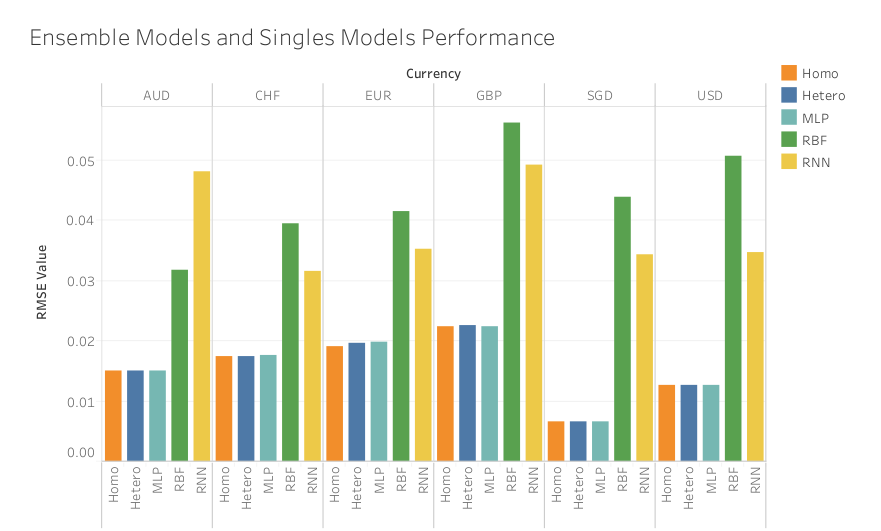
\includegraphics[width=0.5\textwidth]{ensemble_single}
	\caption{Comparison between Ensemble and Single Models Performance}
\end{figure}

\section{Research Contributions}

From the findings discussed above, the homogeneous model trained with 60\% training ratio produce the best optimal model for the all six currency exchange rate. In the current literature, there is only USD to RM exchange rate forecasting using ANNs methods are found. The project contributed by constructing the ensemble model which yield better performance. Moreover, other currency exchange rate such as GBP, EUR, SGD, AUD, and CHF are also forecasted using the same approach with USD to RM exchange rate forecasting.



\section{Future Work}

This project can be extended by increasing the number of predictor order since the project only experimented with predictor number 3 until 10. Moreover, the influence factors such the economic and political situation of the respective exchange rate should put as training inputs parameters. The methods of constructing the ensemble models can be also altered. 


\section{Conclusion}


The performance of ensemble models, homogeneous and heterogeneous models are compared with the single model, which are MLP, RNN, and RBF. The findings conclude that the homogeneous model trained with 60\% training ratio produce the best optimal model for the all six currency exchange rate. For the USD, the optimal homogeneous  performance is 0.012598 RMSE values. This performance is better than current literature performance. Other exchange rates forecasting is also produced reliable performance.

\section{Conclusion}
In this project, an ensemble ANN model is constructed to forecast the exchange rates from Malaysian Ringgit to the six currencies. The two ensemble models are constructed and compared with the single ANN models. The models are trained with three different ratio.  The performance accuracy of USD with homogeneous ensemble models which trained with 60\% training inputs data is better than the current literature performance. The project concludes that the homogeneous ensemble which trained with 60\% training inputs data yield the best accuracy performance for all the currencies. 


% use section* for acknowledgement
\section*{Acknowledgment}


The author would like to express my sincere thanks to my supervisor, Dr. Kannan Ramakrishnan, Faculty of Computing \& Informatics, for his guidance, unconditional supports and encouragement. He has spent considerable amount of time with me for discussions on this project. His guidance, supports, patience, encouragement, constructive suggestions have helped me in a great way to complete this project. 



\ifCLASSOPTIONcaptionsoff
  \newpage
\fi

\begin{thebibliography}{1}

\bibitem {IEEEhowto:beale}

R. Beale and T. Jackson, \emph{Neural Computing-an introduction},\hskip 1em plus
0.5em minus 0.4em\relax CRC Press, 1990.

\bibitem {IEEEhowto:hansen}
L.T Hansen, C. Liisberg and P. Salamon, Ensemble methods for handwritten digit recognition, \emph{Neural Networks for Signal Processing [1992] II., Proceedings of the 1992 IEEE-SP Workshop},  \hskip 1em plus
0.5em minus 0.4em\relax 333-342, IEEE, 1992.

\bibitem {IEEEhowto:giacomel}
F. Giacomel, A. Pereira and R. Galante, Improving financial time series prediction through output classification by a neural network ensemble, \emph{International Conference on Database and Expert Systems Applications},  \hskip 1em plus
0.5em minus 0.4em\relax 331-338, Springer,2015.

\bibitem {IEEEhowto:chan}
T. Chan, C. T. Lye and C. Hooy,  \emph{Forecasting Malaysian Exchange Rate: Do Artificial Neural Networks Work?},  \hskip 1em plus
0.5em minus 0.4em\relax 2010.

\bibitem {IEEEhowto:adhikari}
A. Adhikari and R. Agrawal , \emph{A homogeneous ensemble of artificial neural networks for time series forecasting},  \hskip 1em plus 0.5em minus 0.4em\relax 2013.


\bibitem {IEEEhowto:shao}
M. Shao, X. Zhu, S. Cao, and H. Shen ,An  artificial neural network ensemble method for fault diagnosis of proton exchange membrane fuel cell system, \emph{Energy},  \hskip 1em plus
0.5em minus 0.4em\relax 268-275, Elsevier, 2014.


\bibitem {IEEEhowto:nagahamulla}
H. Nagahamulla, U. Ratnayake, and A. Ratnaweera ,An ensemble of artificial neural networks in rainfall forecasting, \emph{Advances in ICT for Emerging Regions (ICTer), 2012 International Conference on},  \hskip 1em plus
0.5em minus 0.4em\relax 176-181, IEEE, 2012.

\end{thebibliography}

 
 
\end{document}


